\documentclass[aps,rmp, onecolumn]{revtex4}
%\documentclass[a4paper,10pt]{scrartcl}
%\documentclass[aps,rmp,twocolumn]{revtex4}

\usepackage[utf8]{inputenc}
\usepackage{amsmath,graphicx}
\usepackage{color}
%\usepackage{cite}

\newcommand{\Richard}[1]{{\color{red}Richard: #1}}
\newcommand{\LH}{\mathcal{L}}
\newcommand{\rvec}{\mathbf{r}}

\bibliography{bib}

\begin{document}
\title{When to trust phylogeographic inferences?}
\author{Richard Neher}
\date{\today}
\begin{abstract}
    Sometimes.
\end{abstract}

\maketitle
As organisms replicate, they also disperse in space, potentially exploring new habitats.
The reconstruction of ancestral locations and past migrations from sampling locations of extant individuals, typically in combination with genome sequence information to infer the phylogeny, are known as phylogeography.
Phylogeographic methods are implemented in popular evolutionary analysis software such as BEAST \citep{pybus_unifying_2012}.
The underlying model of dispersal is typically diffusive, that is the probability of sampling a descendent at position $\rvec_c$ after time $t$ when the parent was at position $\rvec_p$ is given by
\begin{equation}
    P(\rvec_c| \rvec_p, t) = \frac{1}{4\pi D t}e^{\frac{|r_c - r_p|^2}{4Dt}}
\end{equation}
where $D$ is a diffusion constant with dimensions $\mathrm{length}^2/\mathrm{time}$ and we have assumed a two dimensional space.
Each branch in the phylogeny is adorned with such a diffusive propagator.
Such a diffusive process is the simplest and most natural choice in absence of directed motion or long range migration.
It is also mathematically convenient as unknown ancestral locations can be integrated in closed form and the marginal distribution of each position can be calculated exactly for a fixed tree.
However, it has one major shortcoming: tree topology and branching rates of the tree are independent of the spatial process.
However, these two interact in important ways, for example when a population expands into an uninhabited fertile habitat or a disease spreads in a susceptible population.

At the same time, information in two dimensional sampling locations is low compared to that from high-dimensional sequence space and processes not captured by the diffusive model can potentially result in wrong inferences.
The purpose of this note is to explore how sensitive phylogeographic inferences are to model assumptions and what quantities can be robustly estimated.
My focus here is only on the ability and robustness to estimate dispersal parameter and ancestral locations and I will assume perfect knowledge of the tree and the sampling locations.
So no tree-sampling will be necessary.



In a typically Bayesian phylogeographic inference problem as discussed in \citet{pybus_unifying_2012}, the input data are typically viral genome sequences as well as their sampling times and sampling locations.
Software like BEAST will then sample the posterior distribution of the phylogenetic tree topology, the sampling times and locations of ancestral nodes in the tree, and model parameters like the diffusion constant $D$ and the evolutionary rate $\mu$.
Results can be estimates of the ancestral location of a particular groups of samples, or summary statistics of the dispersal process.
Popular summaries include empirical estimates of the diffusion constant and a so called \emph{dispersal rate}. These are calculated from the displacements along branch $i$ with parent $p_i$ given by $d_i = |\rvec_{p_i} - \rvec_{i}|$ and the elapsed time $\Delta t_i$ as
\begin{equation}
    D_w = \frac{\sum_{i\in B}d_i^2}{4\sum_{i\in B} \Delta t_i} \quad \mathrm{and}  \quad v_w = \frac{\sum_{i\in B} d_i}{\sum_{i\in B} \Delta t_i}
\end{equation}
where $B$ is the set of all branches of the tree.
Effectively $D_w$ divides the sum of all observed squared displacements by the total time elapsed on the tree to obtain and estimate of $D$.
The dispersal rate estimate compares the sum of absolute values of observed displacements to the total time, which has dimensions of a velocity.

Fig.~\ref{fig:D_and_v} shows empirical estimates of $D_w$ and $v_w$ as defined above from simulated data using freely diffusing locations along Kingman or Yule trees.
The diffusion constant $D$ can be estimated robustly from these data, but $v_w$ is not a well defined quantity.
Values of $v_w$ depends strongly on the sample size and there is not ground truth to compare to as there is no parameter with dimensions of a velocity in the model.
That $v_w$ is ill-defined is not surprising: By changing the sample size, the average length of branches changes. Diffusion along each branch results in a displacement of $d_i \sim \sqrt{4Dt_i}$ such that a quantity that depends on $\Delta d_i / t_i \sim 1/t_i^{1/2}$ will change with the time $t_i$ that elapsed along the branch.
Values of $v_w$ are meaningless in this model.

\begin{figure}
    \includegraphics*[width=0.48\textwidth]{figures/kingman_total_dispersal.png}
    \includegraphics*[width=0.48\textwidth]{figures/yule_total_dispersal.png}
    \caption{\label{fig:D_and_v}{\bf Empirical summary statistics of $D$ and ``dispersal rate'' for different sample sizes.}
    While diffusion constant $D$ (equal to 1 in this example) can be robustly estimated from simulation data of the underlying model, the dispersal rate $v_w$ is not a well defined quantity. Its numerical value depends strongly on sample size and there is no ground truth to compare to. This sample size dependence is stronger for Yule trees (right) than Kingman trees (left). }
\end{figure}

\section*{Is the diffusion model consistent?}
Phylogeographic assume that the spatial diffusion process is independent of the branching pattern of the tree and ignores coupling between the two that might arise from density dependent growth rates.
If one simulates a diffusive spatial process in a square of length $L$, the population density shows strong fluctuations whenever the diffusion constant $D<L^2/N$, see Fig.~\ref{fig:heterogeneity}.
$N$ here plays the role of the time to the MRCA of the population.
At $D=0.1L^2/N$, the population distribution is patchy with large areas un-inhabited (Fig.~\ref{fig:heterogeneity} left).
This heterogeneity increases substantially for even lower $D$, when the population is essentially a cloud of width $\sqrt{4DN}\ll L$.

\begin{figure}
    \includegraphics*[width=\textwidth]{figures/heterogeneity_free_diffusion.pdf}
    \caption[short]{\label{fig:heterogeneity}{\bf Population density variation in free diffusion models.}
    When spatial motion is independent of population density, the realized population density in the population will be much larger than biologically plausible. The left panel shows the population density for the case $D = 0.1 L^2/N$ in linear bins of size $L/20$. The right panels shows the standard deviation of the population density for different bin sizes as a function of the diffusion coefficient. For $D>L^2/N$, the heterogeneity approaches the expected value in the well mixed limit. }
\end{figure}

Biological populations spread into areas that support them and will quickly populate fertile areas that are below their carrying capacity.
The simplest model of this process are FKPP waves that model the population density $\phi(x,t)$ as \citep{fisher_wave_1937,KPP1937,hallatschek_life_2010}
\begin{equation}
    \frac{\partial \phi(x,t)}{\partial t} = D\frac{\partial^2 \phi(x,t)}{\partial x^2} + \alpha phi(x,t)(1-\phi(x,t)/\phi_0)
\end{equation}
where $\phi_0$ is the carrying capacity and $\alpha$ is the population growth rate at zero density.
This equation admits solutions with a traveling front, that the population ``invades" the empty territory with velocity $v = 2\sqrt{D \alpha}$.
Note that the model itself does not have an intrinsic velocity.
The speed at which the population invades space is given as compound of diffusion and accelerated growth in regions of low density and only grows like the square root of diffusion constant.
It is thus not clear a priori how estimates of $D$ will be affected by density regulation, even in a constant habitat.

Dependence of growth rate (and thus tree structure) on density is one key element that phylogeographic models ignore because it is very difficult to capture mathematically.
It is, however, fairly straightforward to include this in simulations and these simulations can be used to investigate the nature of phylogeographic inferences when some of the assumptions are violated.
We calculate the population density using a Gaussian kernel with interaction radius $r$
\begin{equation}
    \phi(\rvec) = \sum_{i\in N} \frac{e^{-|\rvec_i - \rvec|^2/2r^2}}{N\sqrt{2\pi r^2}}
\end{equation}
where the sum is over all individuals $i$ in the population of size $N$.
As soon as the interaction radius $r$ is much smaller than the habitat size, this density regulation leads to a more homogeneous population density, see Fig.~\ref{fig:density_reg}.
Diffusion constants estimated from the population remain accurate with moderate overestimation of small diffusion constants.
But with decreasing diffusion, the population fragments into smaller than smaller subpopulations that don't interact or coalesce.
This manifests in an increasing time to the MRCA, see Fig.~\ref{fig:density_reg}.
Spatial location and the coalescence process are thus strongly coupled, in conflict with model assumptions and estimates of population processes are likely biased.

\begin{figure}
    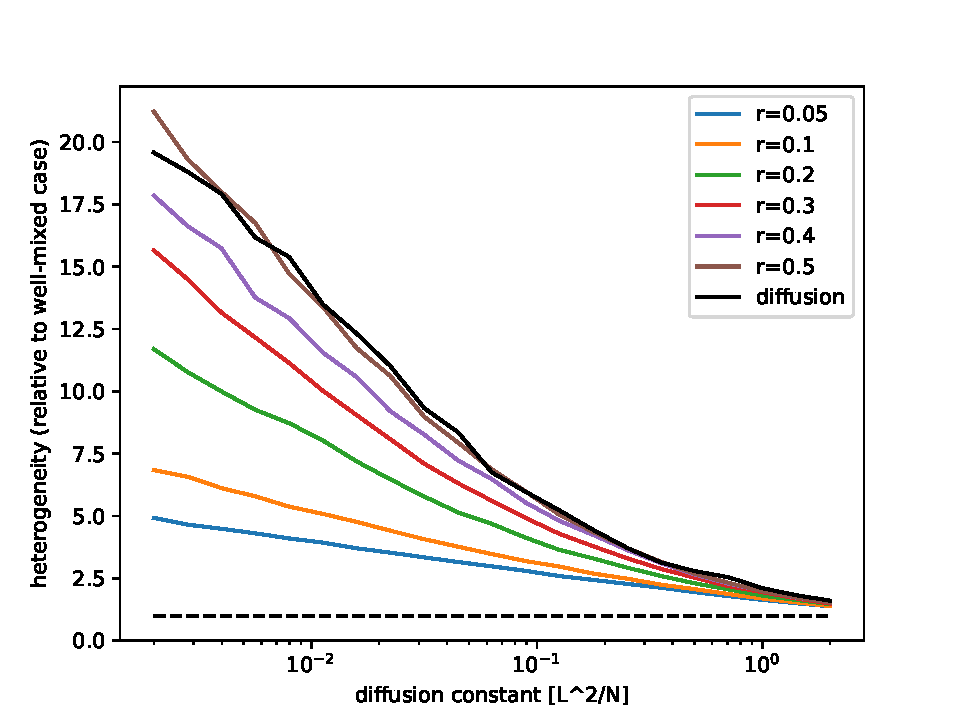
\includegraphics[width=0.48\textwidth]{figures/density_reg_heterogeneity.pdf}
    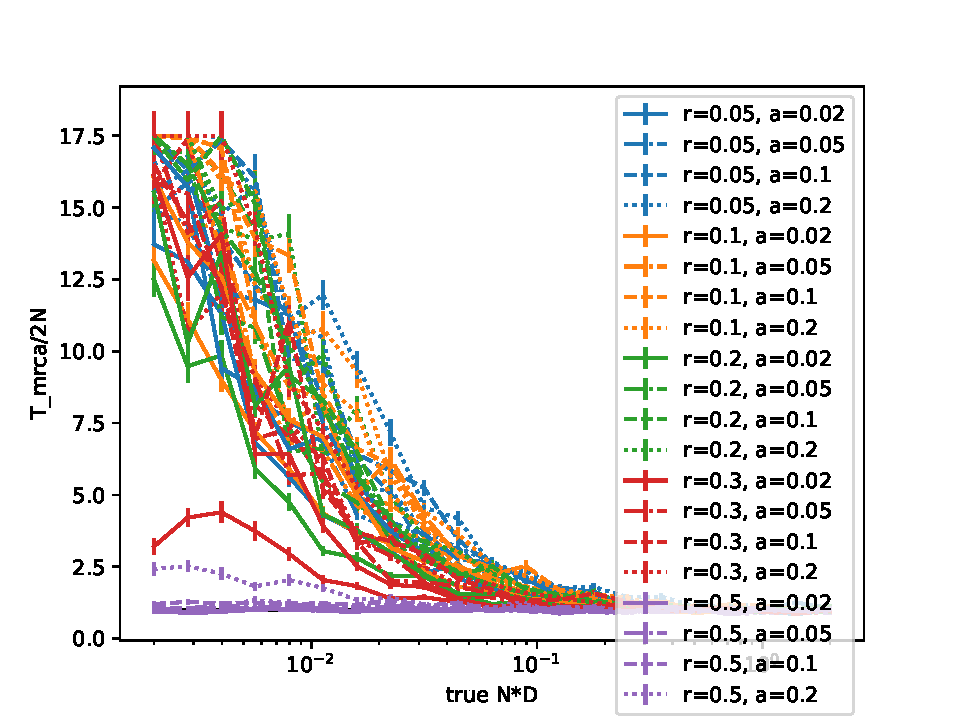
\includegraphics[width=0.48\textwidth]{figures/density_reg_tmrca.pdf}
    \caption{\label{fig:density_reg} {\bf Density regulation reduces fluctuations in density regulation, but results in population fragmentation at low diffusion constants.}}
\end{figure}

The above example assumed a habitat that is constant over times comparable to the time to the most recent common ancestor of the population.
If instead the habitat shifts on shorter time scales, the population has to move and such population movement will skew estimates of dispersal.






\end{document}
